\begin{figure}[h]
	\centering
	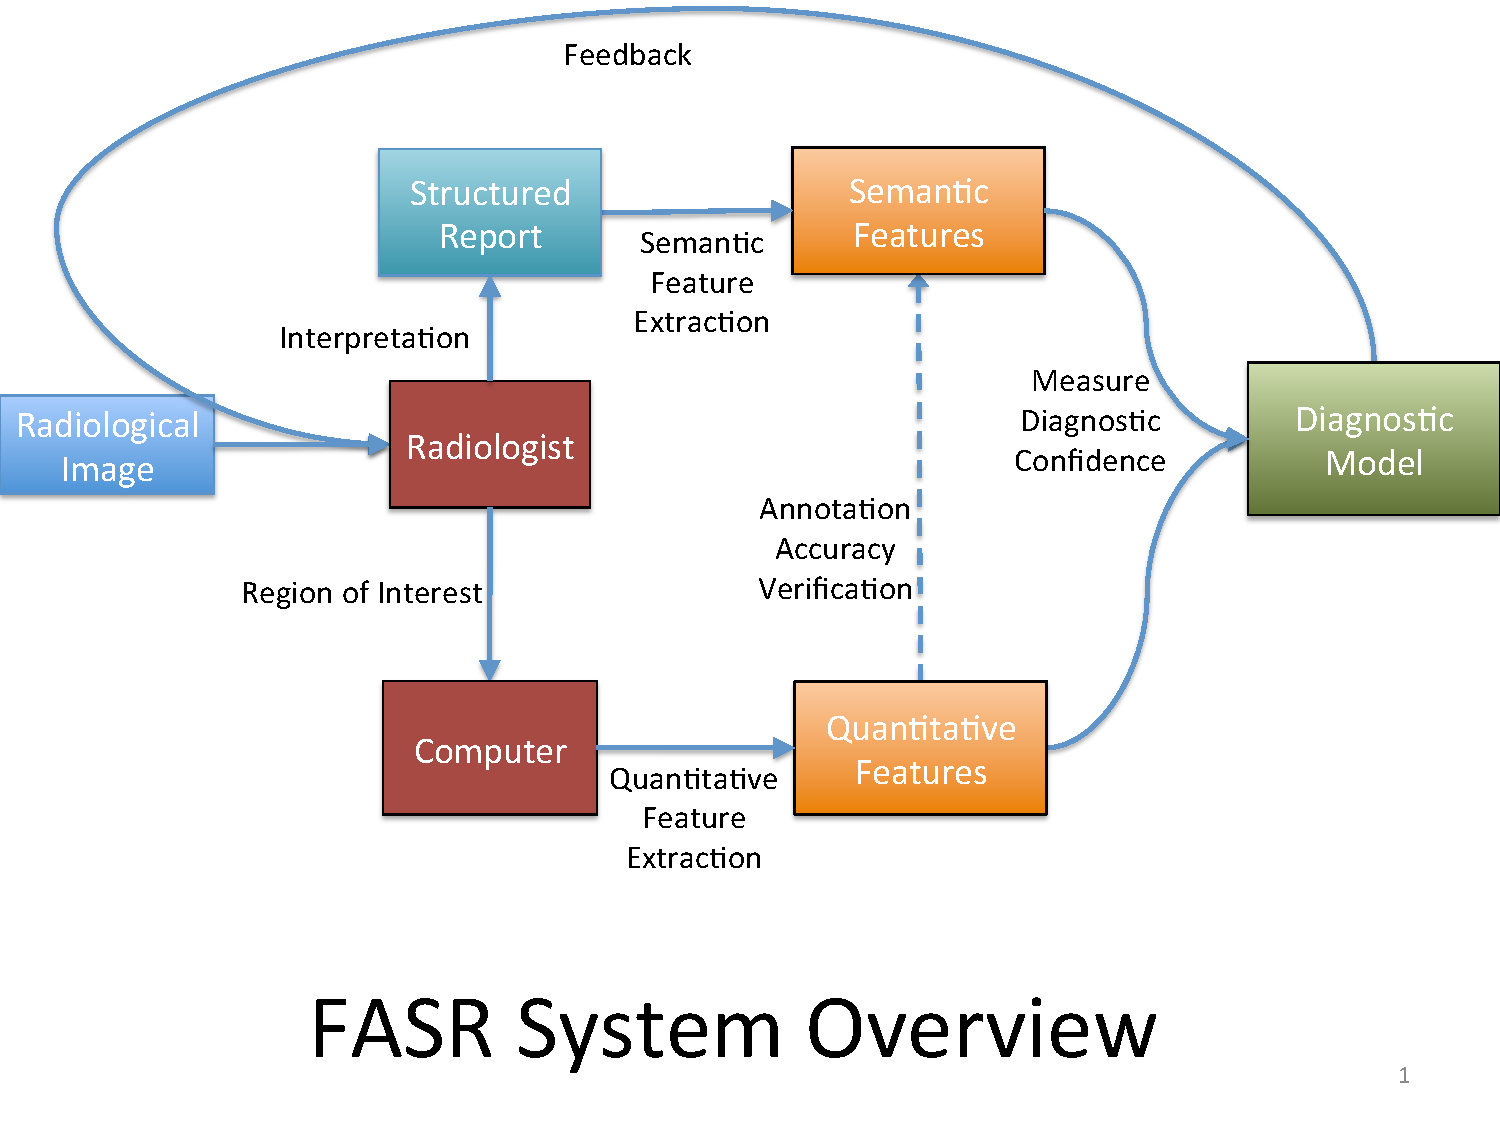
\includegraphics[width=1\linewidth]{fasr_diagram.pdf}
	\caption{Overview of the Fast Adaptive Structured Reporting (FASR) system}
	\label{fig:fasr_diagram2}
\end{figure} 

I have presented a framework to aid in the interpretation of medical images by concurrently analyzing the image and report information while the radiologist independently develops their own interpretation. It then aids in checking that the report is \textbf{correct} by using a predictive framework to estimate the probability of annotations pertaining to the finding. Next it measure how \textbf{complete} the information in the report is by computing a novel \emph{incompleteness score} which is related to the same-decision probability. Finally, the system enforces \textbf{consistency} between the radiologists' evidence and their diagnoses by providing feedback until the gap between both is sufficiently small. 
